\begin{figure}[H]
\centering
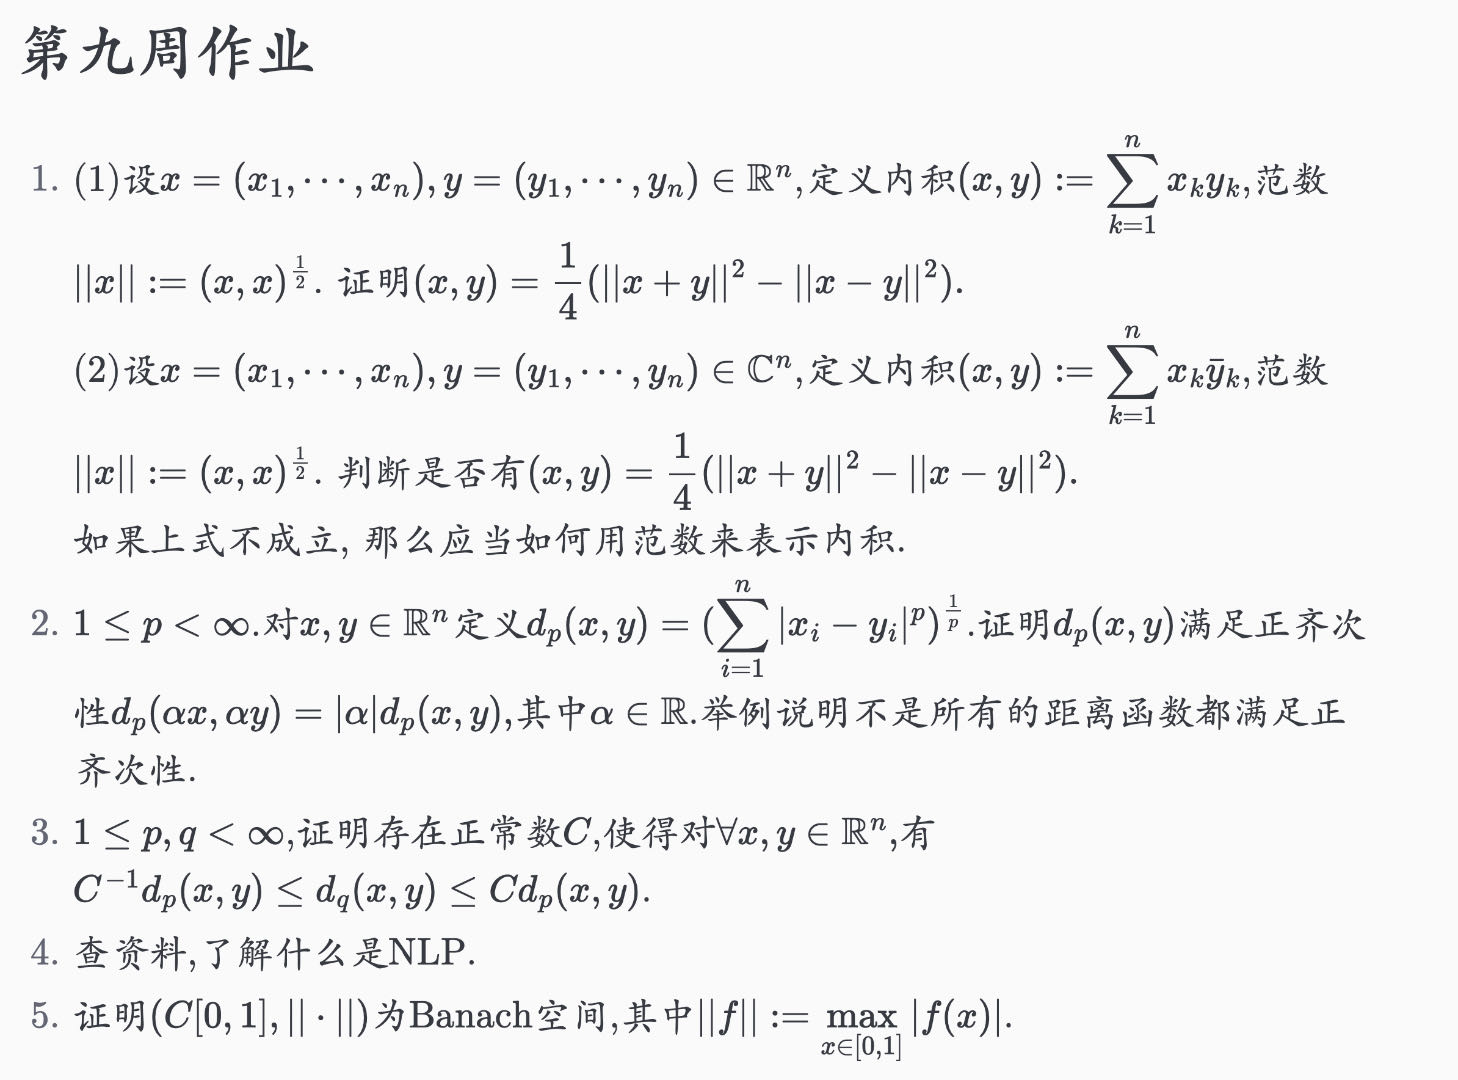
\includegraphics[width=\textwidth]{dcd8d4db5536a3e7deec52448a5ff0b9.jpg}
% \caption{}
\label{}
\end{figure}

\begin{exercise}
\begin{figure}[H]
\centering
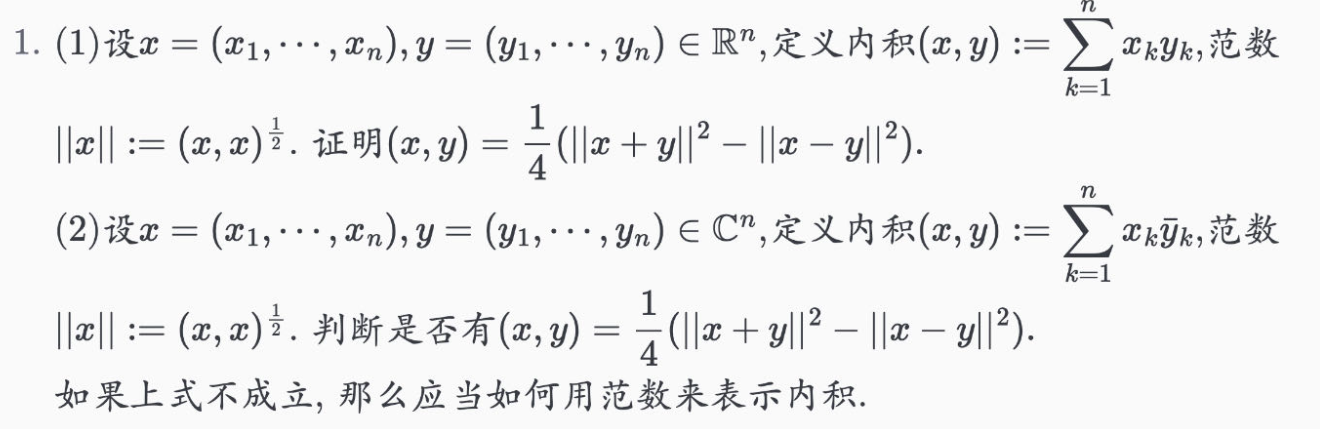
\includegraphics[width=\textwidth]{hw9-2025042812.png}
% \caption{}
\label{}
\end{figure}
\end{exercise}
\begin{proof}
(1)
\[
\begin{aligned}
\lVert x+y \rVert ^2-\lVert x-y \rVert ^2 & =(x+y,x+y)-(x-y,x-y) \\
 & =\sum_{k=1}^{n} (x_k+y_k)^2-\sum_{k=1}^{n} (x_k-y_k)^2 \\
 & =\sum_{k=1}^{n} [(x_k+y_k)^2-(x_k-y_k)^2] \\
 & =\sum_{k=1}^{n} 4x_ky_k \\
 & =4(x,y)
\end{aligned}
\]
(2)
\[
\begin{aligned}
\lVert x+y \rVert ^2-\lVert x-y \rVert ^2 & =\sum_{k=1}^{n} [(x_k+y_k)(\overline{x_k+y_k})-(x_k-y_k)(\overline{x_k-y_k})] \\
 & =\sum_{k=1}^{n} [\lvert x_k \rvert ^2+y_k \overline{x_k}+x_k \overline{y_k}+\lvert y_k \rvert ^2-\lvert x_k \rvert ^2-\lvert y_k \rvert ^2+y_k \overline{x_k}+x_k \overline{y_k}] \\
 & =\sum_{k=1}^{n}  2(y_k \overline{x_k}+x_k \overline{y_k})
\end{aligned}
\]
\[
(x,y)=\sum_{k=1}^{n} x_k \overline{y_k}\neq \frac{1}{4}(\lVert x+y \rVert ^2-\lVert x-y \rVert ^2)
\]
正确的复数极化恒等式为
\[
(x, y)=\frac{1}{4}\left(\|x+y\|^2-\|x-y\|^2+i\|x+i y\|^2-i\|x-i y\|^2\right)
\]
\end{proof}

\begin{exercise}
\begin{figure}[H]
\centering

\includegraphics[width=\textwidth]{hw9-2025042813.png}
% \caption{}
\label{}
\end{figure}
\end{exercise}
\begin{proof}
显然
\[
d_{p}(\alpha x,\alpha y)=\left( \sum_{i=1}^{n}\lvert \alpha x_i-\alpha y_i \rvert ^{p}  \right)^{\frac{1}{p}}=\left( \lvert \alpha \rvert ^{p}\sum_{i=1}^{n} \lvert x_i-y_i \rvert ^{p} \right)^{\frac{1}{p}}=\lvert \alpha \rvert \left( \sum_{i=1}^{n} \lvert x_i-y_i \rvert ^{p} \right)^{\frac{1}{p}}=\lvert \alpha \rvert d_{p}(x,y)
\]
距离函数
\[
d(x,y)=\begin{cases}
0 & x=y \\
1 & x\neq y 
\end{cases}
\]
就不满足正齐次性.
\end{proof}

\begin{exercise}
\begin{figure}[H]
\centering
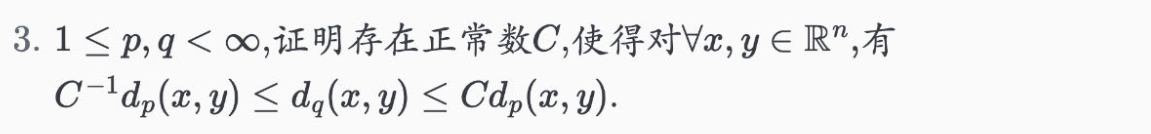
\includegraphics[width=\textwidth]{1-hw9-2025042813.png}
% \caption{}
\label{}
\end{figure}
\end{exercise}
\begin{proof}
For any $p,q$ satisfying $1\leq p,q<\infty$, by Holder's inequality,
\[
\begin{aligned}
d_{q}^{q}(x,y) & =\sum_{i=1}^{n} \underbrace{ \lvert x_i-y_i \rvert ^{q} }_{ =1\cdot\lvert x_i-y_i \rvert ^{q} } \\
 & \leq \left[ \sum_{i=1}^{n} 1^{(p/q)'} \right]^{1/(p/q )'}\cdot\left[ \sum_{i=1}^{n} (\lvert x_i-y_i \rvert ^{q})^{p/q }  \right]^{q/p} \\
 & =n^{p/(p-q)}\cdot d_{p}^{q}(x,y)
\end{aligned}
\]
Thus
\[
d_{q}(x,y)\leq n^{\frac{p}{q(p-q)}}\cdot d_{p}(x,y)
\]
Similarly,
\[
d_{p}(x,y)\leq n^{\frac{q}{p(q-p)}}\cdot d_{q}(x,y)
\]
Pick $C>0$ s.t.
\[
C\geq n^{\frac{p}{q(p-q)}}\qquad \text{and}\qquad C^{-1}\leq n^{-\frac{q}{p(q-p)}}
\]
Then
\[
C^{-1}d_{p}(x,y)\leq d_{q}(x,y)\leq Cd_{p}(x,y)
\]
\end{proof}

\begin{exercise}
\begin{figure}[H]
\centering

\includegraphics[width=\textwidth]{hw9-2025042814.png}
% \caption{}
\label{}
\end{figure}
\end{exercise}
在数学领域中,术语“NLP”通常指的是\textbf{非线性规划} (Nonlinear Programming)。
非线性规划是优化理论的一个分支,研究的是在非线性等式或不等式约束下,如何最小化或最大化一个非线性目标函数的问题。

一个一般的非线性规划问题可以表述为:
最小化(或最大化)$f(x)$
约束条件为:
\[
\begin{aligned}
& g_i(x) \leq 0, i=1, \ldots, m \\
& h_j(x)=0, j=1, \ldots, p \\
& x \in X
\end{aligned}
\]
其中:

\begin{itemize}
	\item $x$ 是决策变量向量。
	\item $f(x)$ 是目标函数,它是一个非线性函数。
	\item $g_i(x)$ 是不等式约束函数,它们可以是线性的或非线性的。
	\item $h_j(x)$ 是等式约束函数,它们可以是线性的或非线性的。
	\item $X$ 是变量的定义域或简单的边界约束,通常是一个凸集。
\end{itemize}

如果目标函数 $f(x)$ 或任何一个约束函数 $g_i(x)$ 或 $h_j(x)$ 是非线性的,那么这个问题就被称为非线性规划问题。作为对比,如果目标函数和所有约束函数都是线性的,那么问题就是线性规划(LP)问题。

非线性规划问题的求解通常比线性规划复杂得多,一般没有统一的,能在多项式时间内找到全局最优解的方法(除非问题具有特定的结构,如凸规划)。常用的求解方法包括梯度下降法,牛顿法,序列二次规划(SQP)等。

请注意,您可能更熟悉在人工智能和计算机科学领域中的“NLP”,它代表的是\textbf{自然语言处理}(Natural Language Processing)。但在数学的优化或运筹学等领域中,“NLP”几乎总是指代非线性规划。

\begin{exercise}
\begin{figure}[H]
\centering

\includegraphics[width=\textwidth]{1-hw9-2025042814.png}
% \caption{}
\label{}
\end{figure}
\end{exercise}
\begin{proof}
Check:

\begin{itemize}
	\item $(C[0,1],\lVert \cdot \rVert)$ is normed linear space.
	\item $(C[0,1],\lVert \cdot  \rVert)$ is complete.
\end{itemize}

To check that $C[0,1]$ is a linear space, we need to verify that it satisfies the axioms of a vector space.

\begin{enumerate}
	\item \textbf{Closure under addition:} If $f, g \in C[0,1]$, then $f+g$ is also continuous on $[0,1]$. Thus, $f+g \in C[0,1]$.
	\item \textbf{Closure under scalar multiplication:} If $f \in C[0,1]$ and $c$ is a scalar, then $cf$ is also continuous on $[0,1]$. Thus, $cf \in C[0,1]$.
	\item \textbf{Commutativity of addition:} For all $f, g \in C[0,1]$, $f(x) + g(x) = g(x) + f(x)$ for all $x \in [0,1]$, so $f+g = g+f$.
	\item \textbf{Associativity of addition:} For all $f, g, h \in C[0,1]$, $(f+g)(x) + h(x) = f(x) + (g+h)(x)$ for all $x \in [0,1]$, so $(f+g)+h = f+(g+h)$.
	\item \textbf{Existence of additive identity:} The zero function $z(x) = 0$ for all $x \in [0,1]$ is continuous on $[0,1]$, so $z \in C[0,1]$. For any $f \in C[0,1]$, $f(x) + z(x) = f(x) + 0 = f(x)$ for all $x \in [0,1]$, so $f+z = f$.
	\item \textbf{Existence of additive inverse:} If $f \in C[0,1]$, then $-f$ is also continuous on $[0,1]$, so $-f \in C[0,1]$. For any $f \in C[0,1]$, $f(x) + (-f(x)) = 0$ for all $x \in [0,1]$, so $f + (-f) = z$.
	\item \textbf{Compatibility of scalar multiplication with field multiplication:} For all scalars $a, b$ and $f \in C[0,1]$, $(ab)f(x) = a(bf(x))$ for all $x \in [0,1]$, so $(ab)f = a(bf)$.
	\item \textbf{Identity element of scalar multiplication:} For all $f \in C[0,1]$, $1 \cdot f(x) = f(x)$ for all $x \in [0,1]$, so $1f = f$.
	\item \textbf{Distributivity of scalar multiplication with respect to vector addition:} For all scalars $c$ and $f, g \in C[0,1]$, $c(f+g)(x) = c(f(x) + g(x)) = cf(x) + cg(x)$ for all $x \in [0,1]$, so $c(f+g) = cf + cg$.
	\item \textbf{Distributivity of scalar multiplication with respect to field addition:} For all scalars $a, b$ and $f \in C[0,1]$, $(a+b)f(x) = af(x) + bf(x)$ for all $x \in [0,1]$, so $(a+b)f = af + bf$.
\end{enumerate}

Since $C[0,1]$ satisfies all the axioms of a vector space, it is a linear space.

\begin{definition}[Normed linear space]
A \textbf{normed linear space} is a linear space $V$ on which there is defined a real-valued function that satisfies
(i) $\|x\| \geq 0$ for all $x \in V$, and $\|x\|=0$ if and only if $x=0$.
(ii) $\|x+y\| \leq\|x\|+\|y\|$ for all $x, y \in V$.
(iii) $\|\alpha x\|=|\alpha|\|x\|$ for all $x \in V$ and all scalars $\alpha$.
\end{definition}
Clearly, $\lVert f \rVert=\max_{x\in[0,1]}\lvert f(x) \rvert\geq0$.
\[
\lVert f+g \rVert =\max_{x\in[0,1]}\lvert f(x)+g(x) \rvert \leq \max_{x\in[0,1]}(\lvert f(x) \rvert +\lvert g(x) \rvert )=\lVert f \rVert +\lVert g \rVert
\]
\[
\lVert \alpha x \rVert =\lvert \alpha \rvert \lVert x \rVert
\]
\begin{definition}[Complete Space]
A metric space $(X, d)$ is called \textbf{complete} if every Cauchy sequence in $X$ converges to a limit that is also in $X$.
\end{definition}
Suppose there is a Cauchy sequence $\{ f_n \}_{n=1}^{\infty}$ of functions in $C[0,1]$. Check that $\{ f_n \}_{n=1}^{\infty}$ converges in $C[0,1]$. Let $f\coloneqq \lim_{ n \to \infty }f_n$, then for any $\epsilon>0$, there exists $N$ s.t. $\forall m,n>N$,
\[
\max_{x\in[0,1]}\lvert f_m(x)-f_n(x) \rvert <\epsilon 
\]
Let $m\to \infty$ then
\[
\max_{x\in[0,1]}\lvert f(x)-f_n(x) \rvert\leq \epsilon
\]
Check that $f\in C[0,1]$. For any $x\in[0,1]$, there exists $\delta>0$, s.t.
\[
\lvert f_n(x)-f_n(y) \rvert <\epsilon \qquad \forall y\in(x-\delta,x+\delta)\cap[0,1],\forall n\geq 1
\]
Then
\[
\lvert f(x)-f(y) \rvert \leq \lvert f(x)-f_n(x) \rvert +\lvert f_n(x)-f_n(y) \rvert +\lvert f_n(y)-f(y) \rvert \leq 3\epsilon
\]
$f\in C[0,1]$, then we are done.
\end{proof}
